
\documentclass[a4paper,12px,twocolumn]{article}

\usepackage[margin=1in]{geometry}
\usepackage{graphicx}
\graphicspath{ {./images/} }

\usepackage{multicol}
\setlength{\columnsep}{1cm}

\begin{document}
\begin{flushleft}
\section{Introduction}

The Fourier transform is used to assess geometric characteristics of a particular spatial
image domain. An image's representation in the Fourier domain is a representation the number
of basis sine and cosine functions of varying frequencies which are present in the image. Because
the image in the Fourier domain is decomposed into into its sinusouidal components, it is easy to
examine the frequencies of the image, and hence influencing the geometric structure in the spatial
domain. This report explains my process of classification of text based of features of the
image extracted from the Fourier domain.

\section{Approach to analysis in the Fourier domain}


To start with, I superimposed the magnitude spectrums of the training data to produce
three graphs which illustrate the geometric characteristics of the letters in the Fourier
space.

\begin{figure}[h!]
  \caption{Fourier transform of T characters}
  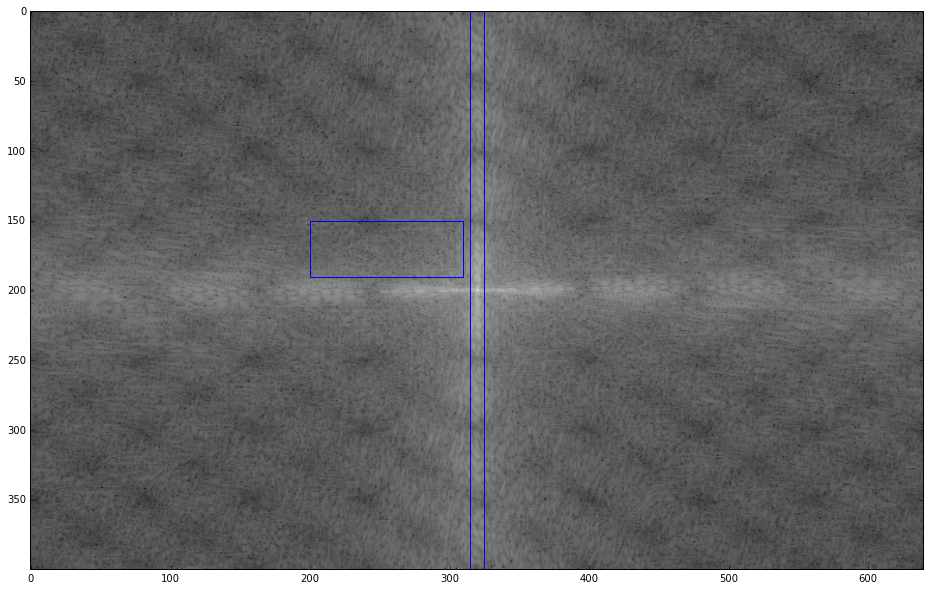
\includegraphics[scale=0.25]{fourierT}
\end{figure}

\begin{figure}[h!]
  \caption{Fourier transform of S characters}
  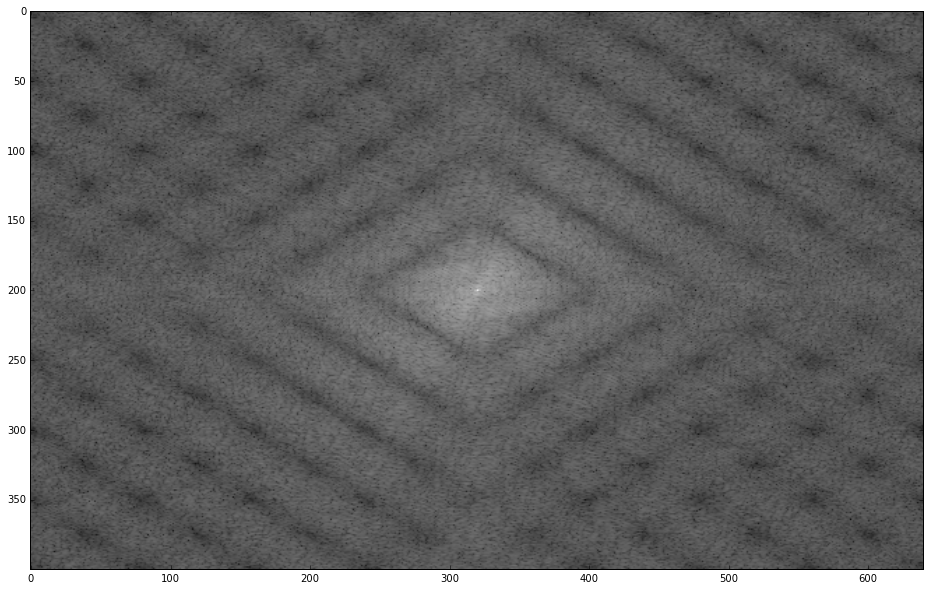
\includegraphics[scale=0.25]{fourierS}
\end{figure}

\begin{figure}[h!]
  \caption{Fourier transform of V characters}
  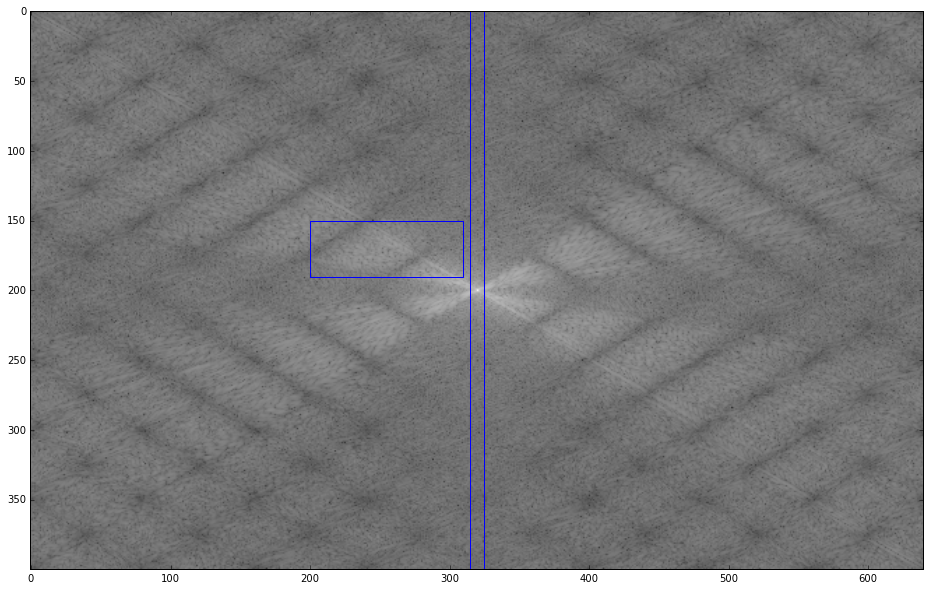
\includegraphics[scale=0.25]{fourierV}
\end{figure}




\smallskip
\newpage

Considering the three Fourier images
\begin{itemize}
    \item Figure 1 shows the average fourier space for the character T, from the image we
    can observe that the power spectrum has high magnitude along the vertical bar passing through the centre,
    this corresponds to the line which forms the top of character T. Similarly, there is another high magnitude bar passing horizontally
    through the centre, corresponding to the vertical part of the character T

    \item Figure 2 shows the average fourier space for the character S, the power spectrum for S shows only small magnitudes for directions
    in exclusively the horizontal or vertical direction, this corresponds to the fact that a regular character S does not change in only
    the vertical or horizontal directions. As seen, the highest magnitudes lie relatively evenly distributed within the central diamond
    region, illustrative of change in both the horizontal and vertical directions, at varying angles.

\end{itemize}


For character V: the power spectrum shows two distinct bands in the lines $ y = x$ and $y = -x$, these
correspond to the two diagonal lines which form the letter V

\smallskip




\section{Choice of features}

    When picking features for the use of classifaction, the aim is to use regions of the
    fourier space which differ the most between fourier spaces for the given characters.
    Leading on from the explanation of the fourier representation of the characters,
    the first feature I picked was a narrow vertical bar covering the height of the images, I reasoned that:
    The narrow vertical bar would measure change in the  horizontal direction of a image, consequently -  the overall
    magnitude spectrum within this region is largest for the letter T. Furthermore, we can observe that the amount of horizontal change
    is next largest in the S character(owing to the top and bottom near horizontal lines which are components of the S character),
    the smallest amount of horizontal change can be seen in the V character, as there is only a very small area at the bottom in which the change
    is purely horizontal.

    \bigskip

    The second feature chosen was a rectangular box in the top left quadrant of the image as shown, I reasoned that
    I should use a feature which did not include change in the vertical or horizontal directly exclusively.
    I reasoned that the T would have the lowest power magnitude in the region mentioned, owing to the fact that a T
    is composed of a vertical and horizontal line placed orthogonally to one another. The next highest magnitude should
    be that of the S, as seen from the Fourier space, S has a high magnitude in the central diamond region. V should have
    the highest magnitude owing to the fact it changes the most in both the horizontal and vertical directions


\section{Results of Fourier Domain analysis and analysis of the classifier}
    Using the features mentioned in the previous section, I computed the sum of the power spectrum in the regions selected
    by the features for each letter.Then, I applied the nearest neighbour procedure with $k=1$ and uniform weighting to the list of
    values produced by the feature extraction, the result is shown in fig.4.
    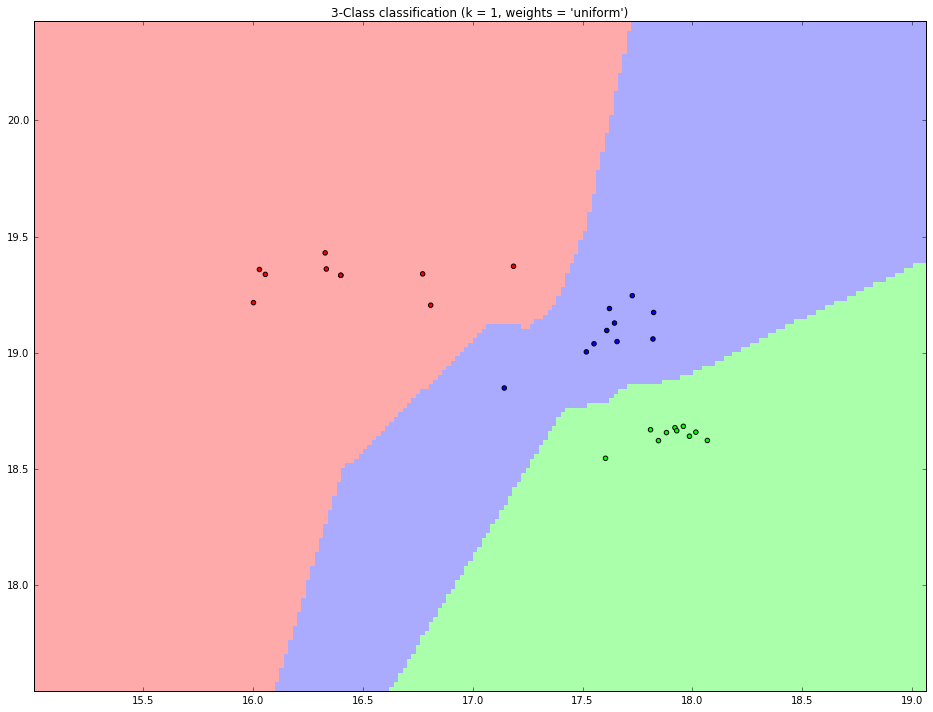
\includegraphics[scale=0.25]{decision}



    The training data produced three regions which correspond to the letters T, V and S. The clustering seems relatively good, except for
    one of the S points. Observing fig * we can see that one S value is far closer to the V decision boundary than the rest. I reasoned that
    the culprit would be an S which had more diagonal information in it than the others, the increased intensity in the $y = -x$ line in the fourier
    space would cause it to increasingly resemble a V. One by one I removed datapoints from the dataset and plotted the resulting nearest neighbour
    classification, I found that the culprit was \textbf{S7}.
    *picture of S7 vs superimposed images of others*

    \bigskip

    To test my classifier, I created 10 new images for each character. The graph below shows the resulting classification for the points. Observing the graph
    we can see that all input Ts have been classified correctly, each T also lies relatively far way from the decision boundary between T and S. Considering
    the next character, Ss have all also been classified correctly for my test data, some of the near the decision boundary for Ss and Ts, this corresponds
    to the more horizontal tops and bottoms of some of the test Ss. my classifier classifier also correctly identified all test V characters, however
    one of test Vs was very close to the decision boundary between S and V, this is a consequence of that particular V being extremly curved.

    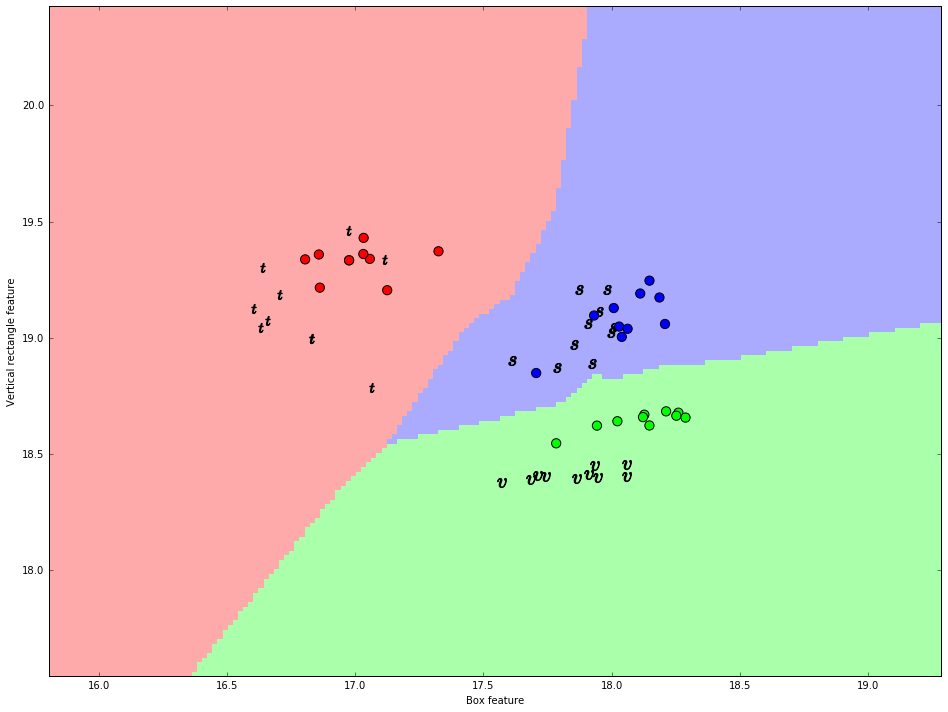
\includegraphics[scale=0.25]{testpoints}

    \bigskip

    Next, I wanted to see how the classifier would cope with extreme cases for some test characters. I created the following
        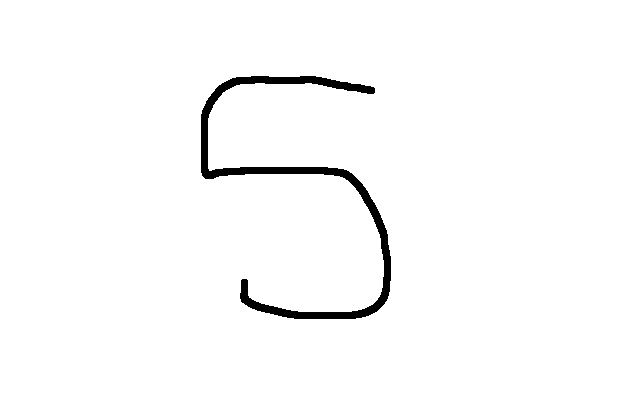
\includegraphics[scale=0.1]{tS11}
        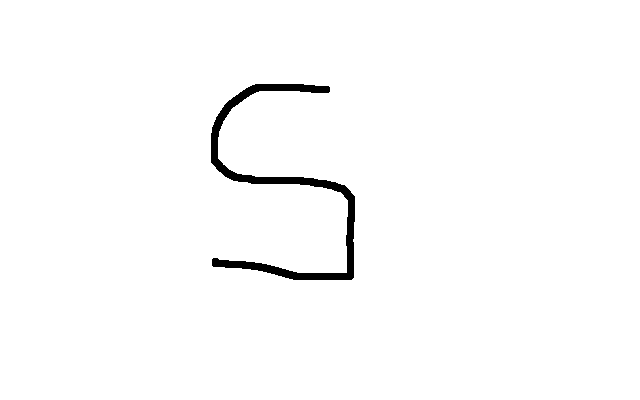
\includegraphics[scale=0.1]{tS12}
        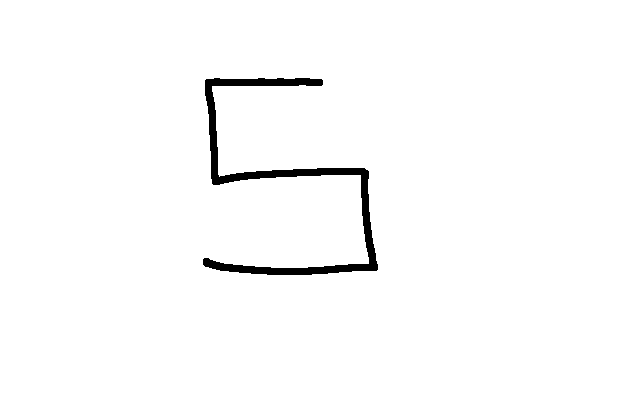
\includegraphics[scale=0.1]{tS13}
        \includegraphics[scale=0.1]{tv11}
        \includegraphics[scale=0.1]{tv12}
        \includegraphics[scale=0.1]{tv13}
        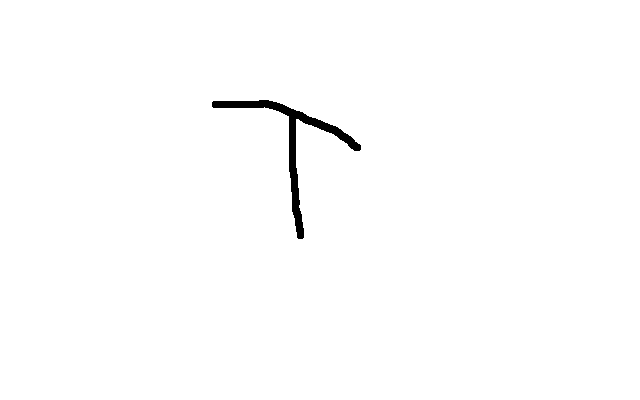
\includegraphics[scale=0.1]{tT11}
        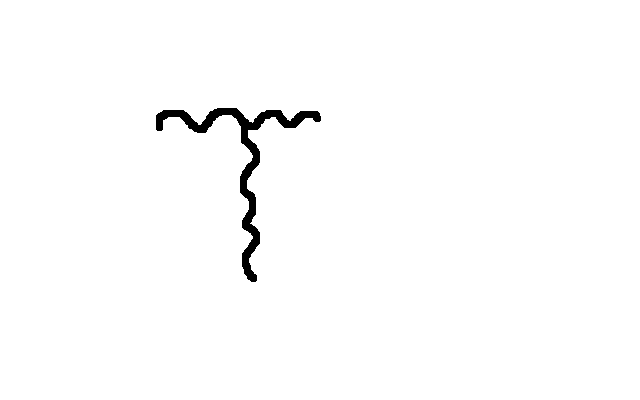
\includegraphics[scale=0.1]{tT12}
        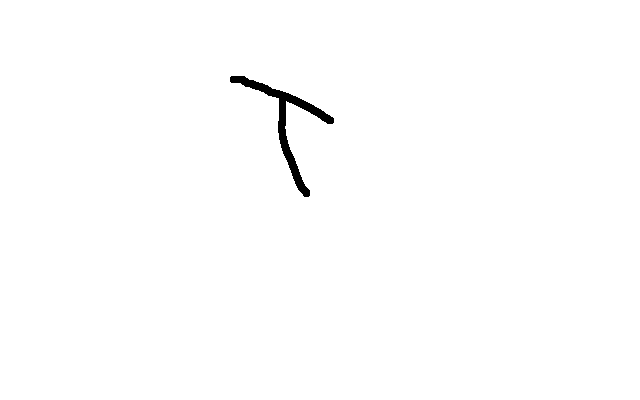
\includegraphics[scale=0.1]{tT13}

        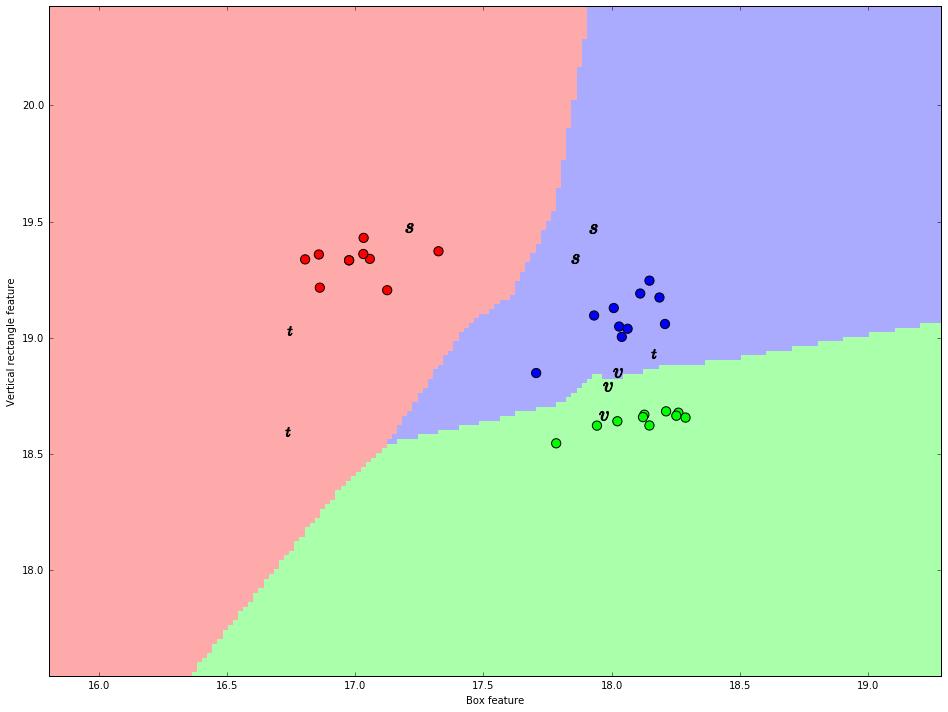
\includegraphics[scale=0.25]{extremechars}



% \section{Analysis of the classifier}

\section{Decision region plots and their angles}

\end{flushleft}



\end{document}
